\documentclass[tikz,border=4pt]{standalone}
\usetikzlibrary{positioning}

\begin{document}
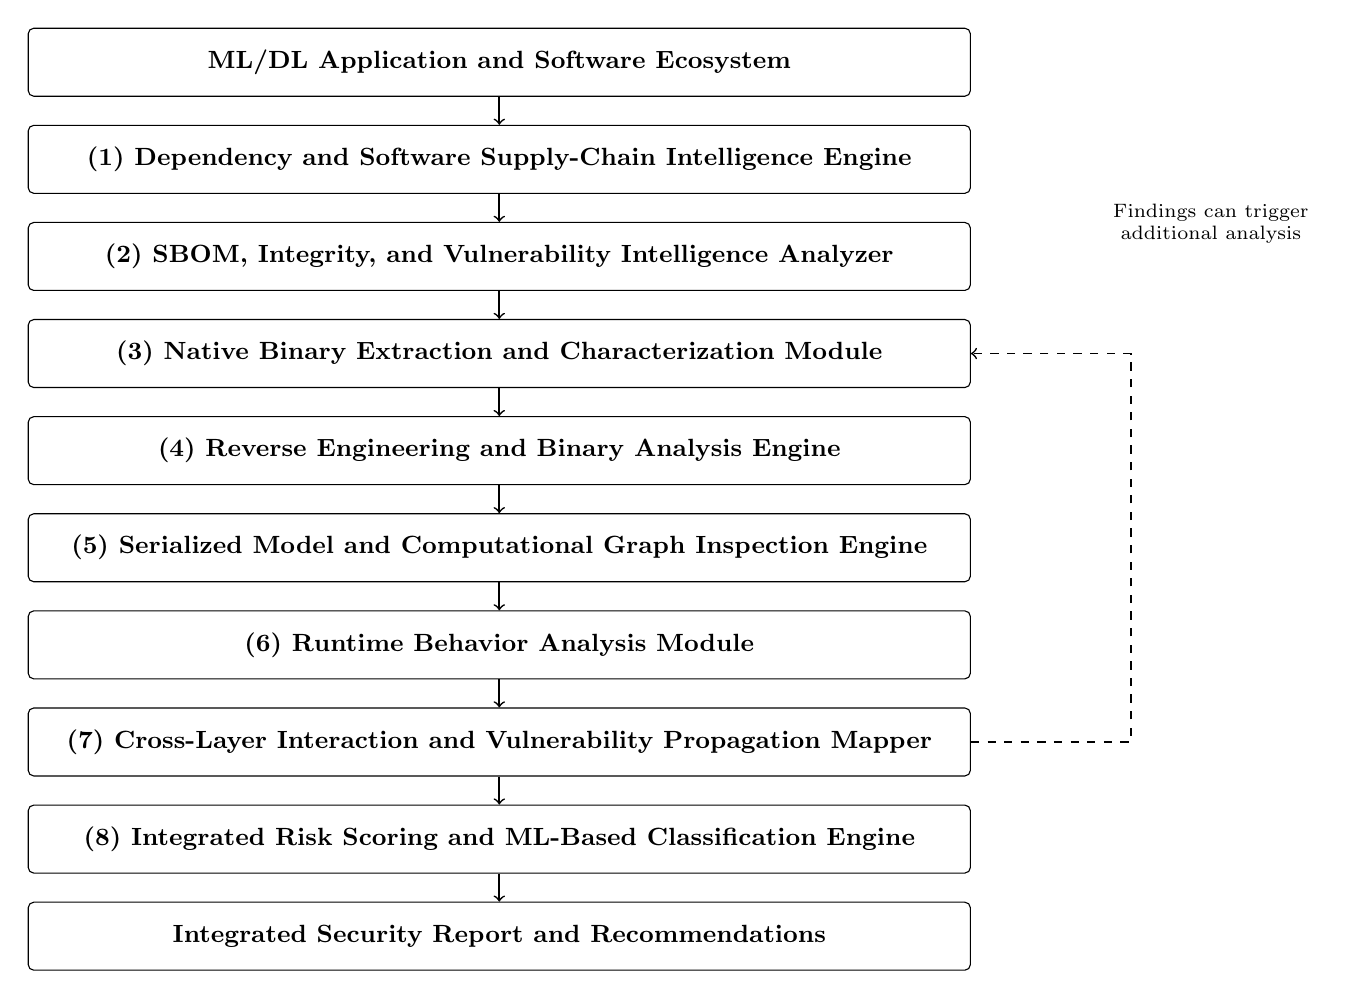
\begin{tikzpicture}[
  component/.style={
    draw,
    rounded corners=2pt,
    text width=4.6in,
    minimum height=0.34in,
    align=center,
    font=\small\bfseries,
    inner sep=4pt
  },
  flow/.style={->, semithick},
  node distance=0.14in
]
\node[component] (ecosystem) {ML/DL Application and Software Ecosystem};
\node[component, below=of ecosystem] (dependency) {(1) Dependency and Software Supply-Chain Intelligence Engine};
\node[component, below=of dependency] (sbom) {(2) SBOM, Integrity, and Vulnerability Intelligence Analyzer};
\node[component, below=of sbom] (binary) {(3) Native Binary Extraction and Characterization Module};
\node[component, below=of binary] (reverse) {(4) Reverse Engineering and Binary Analysis Engine};
\node[component, below=of reverse] (model) {(5) Serialized Model and Computational Graph Inspection Engine};
\node[component, below=of model] (runtime) {(6) Runtime Behavior Analysis Module};
\node[component, below=of runtime] (mapper) {(7) Cross-Layer Interaction and Vulnerability Propagation Mapper};
\node[component, below=of mapper] (risk) {(8) Integrated Risk Scoring and ML-Based Classification Engine};
\node[component, below=of risk] (report) {Integrated Security Report and Recommendations};

\draw[flow] (ecosystem) -- (dependency);
\draw[flow] (dependency) -- (sbom);
\draw[flow] (sbom) -- (binary);
\draw[flow] (binary) -- (reverse);
\draw[flow] (reverse) -- (model);
\draw[flow] (model) -- (runtime);
\draw[flow] (runtime) -- (mapper);
\draw[flow] (mapper) -- (risk);
\draw[flow] (risk) -- (report);

\draw[->, dashed, semithick]
  (mapper.east) -- ++(0.8in,0) |- (binary.east);
\node[align=center, font=\scriptsize]
  at ([xshift=1.2in,yshift=0.65in]binary.east) {Findings can trigger\\additional analysis};
\end{tikzpicture}
\end{document}
